\documentclass[numbers=noenddot]{kurreport}
%preamble
\title{КР.430200.09.03.01.ПЗ}
\providecommand\mytitle{КР. 430200. 09.03.01.ПЗ}
\providecommand\kurtitle{Разработка документации для конструкторско-технологического продукта с программным обеспечением}
% \bibliography{src}

\begin{document}
	\begin{titlepage}
	\changefontsizes[14pt]{14pt}
	\newpage
	\begin{center}
		ФЕДЕРАЛЬНОЕ АГЕНСТВО ЖЕЛЕЗНОДОРОЖНОГО ТАРНСПОРТА \\
		\vspace{14pt}
		Федерально государственное бюджетное образовательное учреждение \\ высшего образования \\
		<<Иркутский государственный университет путей и сообщения>> \\
		(ФГБОУ ВО ИрГУПС) \\
		\vspace{21pt}
		Факультет <<Управление на транспорте и информационнные технологии>> \\
		Кафедра <<Информационные системы и защита информации>>
	\end{center}
	\vspace{28pt}
	\begin{flushleft}
		\begin{tabular}{p{0.47\textwidth}l}
								&  К ЗАЩИТЕ ДОПУСКАЮ				\\
								&  	зав. кафедрой «ИСиЗИ»			\\
								&  	д.т.н., доцент Аршинский Л.В.	\\
		\end{tabular}
	\end{flushleft}
	\vspace{28pt}
	\begin{center}
		\MakeUppercase{\kurtitle}
	\end{center}
	\vspace{-7pt}
	\begin{center}
		Магистерская диссертация \\
	\vspace{14pt}
		\mytitle
	\end{center}
	\vspace{35pt}
	\begin{flushleft}
		\begin{tabular}{p{0.47\textwidth}l}
			КОНСУЛЬТАНТ					&  РУКОВОДИТЕЛЬ ПРОЕКТА		\\
			по нормоконтролю			&  ст. пр. Звонков И.В.		\\
			к.т.р. доцент Матиенко Л.В.	&  							\\
		\end{tabular}
	\end{flushleft}
	\vspace{35pt}
	\begin{flushleft}
		\begin{tabular}{p{0.47\textwidth}l}
								&  ИСПОЛНИТЕЛЬ				\\
								&  студент группы ПИм.1-16-1\\
								&  Арляпов С.В.				\\
		\end{tabular}
	\end{flushleft}
	\vspace{\fill}
	\begin{center}
		Иркутск 2018
	\end{center}
\afterpage{
	\newgeometry{left=3cm,right=1cm,top=1.5cm,bottom=5cm,bindingoffset=0cm}
	\clearpage
	\restoregeometry
}
\end{titlepage}

\setcounter{page}{2}
\renewcommand{\thispagestyle}[1]{}
\tableofcontents
\thispagestyle{empty}

	\chapter*{Задание}\addcontentsline{toc}{chapter}{Задание}
Выполнение курсовой работы направлено на приобретение навыков по разработке технической документации, сопровождающей создаваемый продукт. 
Техническая документация к любому продукту в определенных аспектах основывается на существующих стандартах и нормативных документах, регулирующих то или иное направление функционирования продукта. 
Данные нормативные документы необходимы для обеспечения разработки легального, безопасного, экономически обоснованного и эффективного программного обеспечения. Задача студента составить полное описание продукта и его работы, включающее стадию его разработки и стадию эксплуатации. Курсовая работа должна содержать разделы, освещающие назначение продукта, технические требования к нему и окружению, обеспечивающие надёжность и безопасность работы, конструктивные требования и проектные решения, требования к эксплуатации и условия технического обслуживания, а также технико-экономическое обоснование продукта. 

Для выполнения курсовой работы студент должен ознакомиться с нормативной базой ГОСТов, СНИП и СП, выявить необходимые документы для регулирования функционирования продукта и прописать технические требования и условия для разработки данного продукта.

\chapter*{Введение}\addcontentsline{toc}{chapter}{Введение}
Для внедрения разрабатываемого продукта необходим перечень документов.
Данные документы необходимы для разработки, внедрения и сопровождения разрабатываемого продукта.
В данной курсовой работе разрабатывается перечень документов для охранной системы, а именно:
\begin{enumerate}
\changefontsizes[14pt]{14pt}
	\item Техническое задание;
	\item Техническое предложение;
	\item Технический проект;
	\item Схема функциональная;
	\item Схема структурная;
	\item Схема принципиальная;
	\item Чертёж основания;
	\item Чертёж крышки корпуса;
	\item Чертёж сборочный;
	\item Рисунок печатной платы.
\end{enumerate}

Общеизвестным фактом является то, что с автоматизированными системами рука об руку идёт и программное сопровождение.
Следовательно, в стадии разработки нового продукта следует включить и этапы разработки программного обеспечения.
А также следует разработать требования к программной части продукта и включить в проект программную реализацию.

Для того, чтобы разрабатываемый продукт обладал конкурентоспособностью, уделяют большое внимание на его качество и соответствие принятым стандартам.
Преследуя выше сказанную цель, разрабатываемый продукт подвергают сертификации.
Для успешного завершения процесса разработки и внедрения нового продукта следует ориентироваться на перечень нормативных документов, например:
\begin{itemize}
\changefontsizes[14pt]{14pt}
	\item ГОСТ 34.602 89\cite{gost89};
	\item ГОСТ 34.601.90\cite{gost90}:
	\item ГОСТ 34.603.92\cite{gost92};
	\item ГОСТ 2.114-95\cite{gost95};
	\item ГОСТ Р 53736-2009\cite{gost09}.
\end{itemize}

Сейчас существует разнообразное множество стандартов и рекомендаций, которые находятся в свободном доступе.
В процессе выполнения данной курсовой работы следует ознакомиться с некоторым перечнем нормативных документов и получить 
навыки в разработки продуктов с программным обеспечением.

	\chapter{Техническое задание}
	\section{Обоснование для проведения работ}
		Задание преподавателя.
	\section{Исполнитель работ}
		Студент ИрГУПС ФУТиИT группы ПИм-16 Арляпов С.В.
	\section{Цель выполнения работ}
		Разработать устройство охранной сигнализации, предназначенное для контроля, мониторинга и управления территориально-распределенными объектами муниципальных и ведомственных образований с целью увеличения безопасности.
	\section{Назначение продукции}
		Устройство будет обеспечивать сбор, обработку, передачу и представление в заданном виде служебной информации и информации о проникновении (попытки проникновения).
	\section{Технические требования}
		\subsection{Состав продукции}
		 	\begin{enumerate}
				\item Основной блок устройства обработки информации;
				\item Датчики «Рапид 3» - 3 штуки;
				\item Витая пара – 1 км;
				\item Вилки «RJ-45» - 5 штук;
				\item Эксплуатационная документация.
			\end{enumerate}
		\subsection{Требования к показателям назначения}
			\subsubsection{Выполняемые функции}
				Разрабатываемое устройство должно обеспечивать в режиме реального времени:
				\begin{enumerate}
					\item сбор данных;
					\item обработку данных;
					\item оповещение оператора.
				\end{enumerate}
			\subsubsection{Нормы и количественные показатели}
				\begin{itemize}
					\item Время реакции не менее 1 секунды.
					\item Время срабатывания механизма оповещения не менее 30 секунд.
					\item Дальность обнаружения датчиком не менее 15 метров.
				\end{itemize}
			\subsubsection{Технические характеристики (параметры)}
				Максимальное количество подключаемых датчиков не менее 4 штук.

				Максимальная длина кабеля, подключающего датчик к устройству, 400 метров
			\subsubsection{Требования к совместимости}
				Особых требований не предъявляется.

			\subsubsection{Требования по мобильности}
				Разрабатываемое изделие должно быть выполнено в стационарном исполнении.
		\subsection{Требования к электропитанию}
			Электропитание осуществляется по первой категории надежности от однофазной (трехфазной) сети переменного тока 220В, 50Гц, от отдельной группы электрощита, находящегося в охраняемом помещении.
		\subsection{Требования надежности}
			\subsubsection{Требования по безотказности}
				Разрабатываемое устройство должно удовлетворять следующим требованиям:
				\begin{itemize}
					\item вероятность безотказной работы 0,95, не менее;
					\item средняя наработка на отказ 50000 часов, не менее;
					\item среднее время восстановления 1 час, не более.
				\end{itemize}
			\subsubsection{Требования по долговечности}
				Разрабатываемое устройство должно удовлетворять следующим требованиям: срок службы до списания 8 лет, не менее.
			\subsubsection{Критерии отказов и предельного состояния изделия}
				Отказом разрабатываемого изделия считают невыполнение функций, заданных требованиями п.5.2.1 настоящего технического задания.
		\subsection{Конструктивные требования}
			\subsubsection{Конструктивное исполнение входящих в разрабатываемое устройство должно обеспечивать:}
				\begin{enumerate}
					\item Удобство эксплуатации;
					\item Возможность ремонта.
				\end{enumerate}
				\subsubsection{Разрабатываемое изделие должно иметь моноблочную конструкцию.}
				\subsubsection{Разрабатываемое изделие должно соответствовать следующим требованиям:}
					\begin{enumerate}
						\item Размеры:
							\begin{enumerate}
								\item Габаритные - 450х450х160 мм, не более;
								\item Установочные - 500х500х210 мм, не более.
							\end{enumerate}
						\item Масса - 2 кг, не более.
						\item Устройство крепится на вертикальную поверхность с помощью винтовых соединений.
						\item Тип кабеля – витая пара.
						\item Тип порта - RJ-45.
						\item Разрабатываемое изделие должно иметь максимальную длину кабеля, подключающего датчик к устройству, 400 метров.
					\end{enumerate}
					\subsubsection{Покрытия должны обеспечивать необходимую коррозионную стойкость, надежную работу и декоративный вид разрабатываемого изделия при эксплуатации и при хранении.}
					\subsubsection{Оборудование не должно требовать доступа сзади при монтаже, подводке кабеля и обслуживании.}
					\subsubsection{Внешние электрические разъемы должны иметь маркировку, позволяющую определить их назначение.}
					\subsubsection{Электрическая схема должна быть выполнена на единой печатной плате. Монтаж должен осуществляться с помощью методов групповой пайки.}
		\subsection{Требования по эргономике и технической эстетике}
			Кодирование и компоновка средств отображения информации, органов управления на пульте управления, цветовое оформление лицевых панелей пульта разрабатываемого изделия должны обеспечивать безошибочность и быстродействие операторов, удобство и безопасность работы в любое время суток.  Необходимо предусмотреть независимое автономное питание, обеспечивающее работу ПКП и извещателей в течении не менее чем 24 часов в дежурном режиме и в течении не менее чем 3 часов в режиме «тревога».
		\subsection{Требования к эксплуатации, удобству технического обслуживания и ремонта}
			\subsubsection{Требования к стойкости к внешним воздействующим факторам}
				1) Разрабатываемое изделие должно быть стойким, устойчивым и прочным к воздействию климатических факторов в соответствии с таблицей \ref{taskt1}:
				\renewcommand{\arraystretch}{1.5}
\begin{longtable}[t]{@{\extracolsep{\fill}}|l|l|l|l|}
	\caption{Воздействие климатических факторов} \label{taskt1} \\
	\hline
	{\No} & \shortstack{Наименование\\ воздействующего\\ фактора \vspace{27pt}}
			  & \shortstack{Характеристика\\ воздействующего\\ фактора \vspace{25pt}}
				& \shortstack{\\ Максимальное\\ значение (диапазрн\\ возможных измерений)\\ воздействующего\\ фактора}   \\ \hline
	\multicolumn{4}{|c|}{Стойкость}    \\ \hline
	1     & \shortstack{\\ Температура\\ окружающей среды} & Градусов цельсия                                                             & 5 до 35     \\ \hline
	2     & Влажность воздуха                           & \shortstack{\\ Относительная\\ влажность при\\ температуре $25^{\circ}$, \%}             & до 70       \\ \hline
	3     & Атмосферное давление                        & Па (мм рт. ст.)                                                              & 630 до 800  \\ \hline
	\multicolumn{4}{|c|}{Устойчивость}   \\ \hline
	4     & \shortstack{\\ Температура\\ окружающей среды} & Градусов цельсия                                                             & 40          \\ \hline
	6     & Влажность воздуха                           & \shortstack{\\ Относительная\\ влажность при\\ температуре $25^{\circ}$, \%}             & до 80       \\ \hline
	9     & Атмосферное давление                        & Па (мм рт. ст.)                                                              & 800 до 900  \\ \hline
	\multicolumn{4}{|c|}{Прочность}   \\ \hline
	7     & \shortstack{\\ Температура\\ окружающей среды} & Градусов цельсия                                                             & 50          \\ \hline
	8     & Влажность воздуха                           & \shortstack{\\ Относительная\\ влажность при\\ температуре $25^{\circ}$, \%}             & до 90       \\ \hline
	9     & Атмосферное давление                        & Па (мм рт. ст.)                                                              & 900 до1000  \\ \hline
\end{longtable}


				2) Разрабатываемое изделие должно быть устойчивым к воздействию механических факторов в соответствии с таблицей \ref{taskt2}:
				\begin{longtable}[t]{@{\extracolsep{\fill}}|l|l|l|l|}
	\caption{Воздействие климатических факторов} \label{taskt2} \\ \hline
	{\No} & \shortstack{Наименование\\ воздействующего\\ фактора \vspace{27pt}}
			  & \shortstack{Характеристика\\ воздействующего\\ фактора \vspace{25pt}}
				& \shortstack{\\ Максимальное\\ значение (диапазрн\\ возможных измерений)\\ воздействующего\\ фактора}   \\ \hline
	\endfirsthead
	\caption* {Продолжение таблицы \ref{taskt2}}\\ \hline
	{\No} & \shortstack{Наименование\\ воздействующего\\ фактора \vspace{27pt}}
			  & \shortstack{Характеристика\\ воздействующего\\ фактора \vspace{25pt}}
				& \shortstack{\\ Максимальное\\ значение (диапазрн\\ возможных измерений)\\ воздействующего\\ фактора}   \\ \hline \endhead
	1     & \shortstack{\\ Синусоидальная\\ вибрация} & \shortstack{\\ диапазон частот, Гц}  & $0,5 - 200 * 10^8$     \\ \hline
	2     & \shortstack{\\ Случайная\\ вибрация} & \shortstack{\\ диапазон частот, Гц}       &  $0,5 - 200 * 10^{20}$    \\ \hline
	3     & \shortstack{\\ Удары\\ многократного\\ действия} & \shortstack{\\ максимальная амплитуда\\ ускорения, $m*c^2, (g)$ } & 10     \\ \hline
	4     & \shortstack{\\ Удары\\ одиночного\\ действия} & \shortstack{\\ максимальная амплитуда\\ ускорения, $m*c^2, (g)$ } & 20     \\ \hline
	5     & \shortstack{\\ Линейное\\ ускорение} & \shortstack{\\ максимальная амплитуда\\ ускорения, $m*c^2, (g)$ } & 30     \\ \hline
\end{longtable}


			\subsubsection{Требования к эксплуатационным показателям}
				\begin{enumerate}
					\item Разрабатываемый Комплекс должен обеспечивать циклическую работу со следующими параметрами цикла: время загрузки – 30 мин., время обработки – 10 час., время выгрузки – 30 мин., время подготовки – 10 мин.
					\item Должен быть обеспечен режим работы от аварийного источника питания.
					\item Периодическое техническое обслуживание разрабатываемого изделия должно проводиться не реже одного раза в год.
					\item Периодическое техническое обслуживание должно включать в себя обслуживание всех датчиков.
					\item К обслуживанию комплекса должны допускаться лица, имеющие допуск к работе с электроустановками напряжением до 220 В.
					\item Гарантийный срок разрабатываемого Комплекса должен составлять 5 лет, не менее.
				\end{enumerate}
			\subsubsection{Требования по ремонтопригодности}
				\begin{enumerate}
					\item Обслуживание и ремонт разрабатываемого Изделия должны производиться без применения специальных инструментов."
					\item Требования к ЗИП
						\begin{enumerate}
							\item Комплект ЗИП должен включать запасные части, необходимые для ремонта и поддержания работоспособного состояния разрабатываемого изделия в течение одного года.
							\item В комплект ЗИП должны входить дополнительные датчики и вилки RJ-45.
						\end{enumerate}
				\end{enumerate}
		\subsection{Требования безопасности}
			\subsubsection{Условия работы персонала разрабатываемой Системы должны соответствовать санитарным нормам по СанПиН 2.2.2/2.4.1340-03 \cite{sanpin}.}
			\subsubsection{Требования безопасности при монтаже, наладке, эксплуатации, обслуживании и ремонте разрабатываемого Комплекса должны быть приведены в эксплуатационной документации.}
		\subsection{Требования к упаковке и маркировке}
			\subsubsection{Требования к упаковке}
				Упаковка должна быть выполнена из картона материалов и обеспечивать защиту от ударных воздействий.
			\subsubsection{Требования к маркировке}
				Надписи, цифры, буквы и знаки, нанесенные при маркировке, должны быть хорошо видны, и сохранять четкость в течение всего срока эксплуатации.
				Маркировка упаковки для транспортирования должна содержать основные, дополнительные, информационные надписи и манипуляционные.
		\subsection{Требования к консервации, хранению и транспортированию}
			\subsubsection{Условия хранения}
				Изделие должно храниться в упакованном виде в отапливаемых и вентилируемых помещениях при температуре от 5 до 35 °С и относительной влажности воздуха не выше 80\% (при температуре 25 °С) при отсутствии в этих помещениях конденсации влаги, паров химически активных веществ и источников электромагнитных полей.
			\subsubsection{Срок хранения}
				Срок хранения разрабатываемого изделия в условиях отапливаемых хранилищ в соответствии с паспортными данными на аппаратуру, но не менее 8 лет.
			\subsubsection{Условия транспортирования:}
				\begin{itemize}
					\item Температура окружающей среды: от минус 50 до 50 °С;
					\item Относительная влажность до 95 \% при температуре 30 °С;
					\item Атмосферное давление от 84 до 107 кПа (от 630 до 800 мм рт. ст.);
					\item Воздействие ударных нагрузок многократного действия с пиковым ускорением не более 15g (147 м/с2) при длительности действия ударного ускорения 10–15 мс.
				\end{itemize}
				\subsubsection{Гарантийный срок хранения разрабатываемого прибора в заводской упаковке в отапливаемом помещении}
					Не менее одного года.
		\subsection{Требования стандартизации, унификации и каталогизации}
			Особых требований не предъявляется.
	\section{Требования по видам обеспечения}
		\subsection{Требования по метрологическому обеспечению}
			Особых требований не предъявляется.
		\subsection{Требования по программному обеспечению}
			\subsubsection{Назначение}
				Программное обеспечение должно предоставлять возможность работы с информацией,
					то есть реализовывать основные функции при работе с информацией, а именно:
				\begin{itemize}
					\item Сбор;
					\item Хранение;
					\item Передачу.
				\end{itemize}
			\subsubsection{Нормативные документы}
				При разработке и вводе в эксплуатацию программного обеспечения
				Исполнитель должен руководствоваться требованиями следующих
				нормативных документов Госстандарта:
				\begin{itemize}
					\item ГОСТ 34.601.90 – стандарт, устанавливающий стадии и этапы создания АС, а также содержание работ на каждом этапе \cite{gost90};
					\item ГОСТ 34.603.92 – стандарт, устанавливающий виды испытаний АС и общие требования к их проведению \cite{gost92}.
				\end{itemize}
	\section{Технико-экономические требования}
		\subsection{Основные технико-экономические требования}
			Разрабатываемый продукт должен обеспечить:
			\begin{itemize}
				\item стимулирование внедрения и использования эффективных, оптимальных по стоимости, охранных систем;
				\item создание унифицированного решения для организации информационного взаимодействия между подразделениями.
			\end{itemize}
			Внедрение создаваемой в рамках разработки научно-технической продукции должно обеспечивать следующие социально-экономические эффекты:
			\begin{itemize}
				\item сокращение сроков разработки 3 месяца;
				\item уменьшение технического риска при реализации передовых технических решений в сфере охраны.
			\end{itemize}
			Разрабатываемая продукция должна быть ориентирована на коммерческое применение в следующих областях:
			\begin{itemize}
				\item системы охраны, мониторинга и управления;
				\item системы автоматизации организаций, связанных с охраной.
			\end{itemize}

	\section{Наименование этапов и выполняемых работ}
		\begin{enumerate}
			\item Техническое предложение:
				\begin{enumerate}
					\item Выбор датчиков;
					\item Выбор структурной схемы;
					\item Выбор оптимального варианта реализации;
					\item Разработка и согласование с преподавателем комплекта технической документации, разрабатываемой в рамках договора;
					\item Разработка ТД в соответствии с согласованном комплектом.
				\end{enumerate}
			\item Технический проект:
				\begin{enumerate}
					\item Разработка технического проекта, в том числе:
						\begin{itemize}
							\item Разработка конструктивных решений Комплекса и его составных частей:
								\begin{itemize}
									\item Разработка чертежей;
									\item Разработка функциональной и принципиальной схемы.
									\item Создание рисунка печатной платы.
								\end{itemize}
							\item Выполнение необходимых расчетов для технических решений, обеспечивающих показатели надежности.
						\end{itemize}
					\item Разработка эксплуатационной документации в соответствии с согласованном перечнем.
				\end{enumerate}
		\end{enumerate}

	\chap{Техническое предложение}
	\section{Сравнительный анализ вариантов реализации}
		Прибор сравнивает значение с датчиков и заданное значение, результаты передаются на выходы управляющего устройства.

		Различные варианты реализации представлены на рисунках \ref{offerp1} и \ref{offerp2}.
		\begin{figure}[ht!]
			\centering
			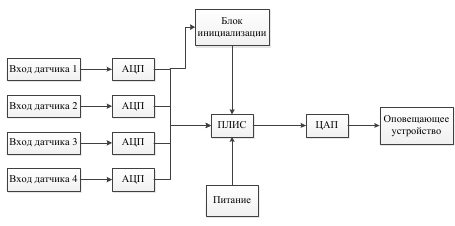
\includegraphics[width=150mm]{src/pictures/offerp1.png}
			\caption{Структурная схема на ПЛИС}\label{offerp1}
		\end{figure}
		\begin{figure}[ht!]
			\centering
			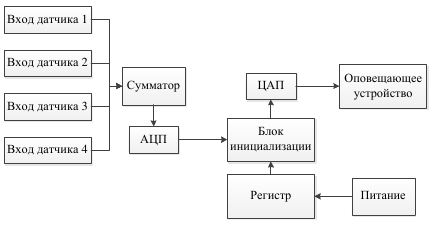
\includegraphics[width=150mm]{src/pictures/offerp2.png}
			\caption{Структурная схема на компараторе и микроконтроллере}\label{offerp2}
		\end{figure}

		Сравнение вариантов реализации представлено в таблице \ref{offert1}.
		\begin{longtable}[t]{@{\extracolsep{\fill}}|l|@{\hskip-14pt}p{0.3\textwidth}|@{\hskip-14pt}p{0.3\textwidth}|}
	\caption{Сравнение реализаций} \label{offert1} \\ \hline
	Вид & На ПЛИС & На регистре и компораторе \\ \hline
	\endfirsthead
	\caption* {Продолжение таблицы \ref{offert1}}\\ \hline
	Вид & На ПЛИС & На регистре и компораторе \\ \hline
	\endhead
	Структура	&
		1) ПЛИС хранит установленные настройки и суммирует значения датчиков. 

		2) Сравнение установленных настроек и показателей датчиков производится посредством ПЛИС. 

		3) Результат сравнения преобразуется из цифрового сигнала в аналоговый.
					&
		1) Цифровой регистр хранит установленные настройки. 

		2) Значения с датчиков проходят через сумматор. 

		3) Сравнение установленных настроек, хранимых в регистре, и показателей датчиков производится с помощью компаратора. 

		4) Выходная информация с компаратора преобразуется в аналоговый сигнал.
		\\ \hline
	Преимущества	&
		Низкое энергопотребление
					&
		Простой ремонт, низкая стоимость
		\\ \hline
	\shortstack{\\ Примерная\\ стоимость}	&
		1750
					&
		1200
		\\ \hline
\end{longtable}


	\section{Выбор датчиков}
		Датчик движения - это устройство для получения информации о состоянии контролируемой им системы, преобразующее данные об изменении характеристик исследуемой области в сигнал, удобный для дальнейшего использования.
		\subsection{Выбор типа датчиков}
			Под понятием «датчик движения» или «датчик присутствия», часто скрываются устройства совершенно разного принципа действия, выполняющие единую задачу, только различными способами.

			В настоящее время наибольшее распространение получили следующие виды датчиков движения:
			\begin{itemize}
\changefontsizes[14pt]{14pt}
				\item Инфракрасные датчики движения (ИК);
				\item Ультразвуковые датчики движения (УЗ);
				\item Микроволновые датчики движения (СВЧ).
			\end{itemize}
			Плюсы и минусы представлены в таблице \ref{offert2}.
			{
\changefontsizes[14pt]{14pt}
\begin{longtable}[t]{@{\extracolsep{\fill}}|l|@{\hskip-14pt}p{0.3\textwidth}|@{\hskip-14pt}p{0.3\textwidth}|}
	\caption{Сравнение видов датчиков} \label{offert2} \\ \hline
	Вид & Преимущества & Недостатки \\ \hline
	\endfirsthead
	\caption* {Продолжение таблицы \ref{offert2}}\\ \hline
	Вид & Преимущества & Недостатки \\ \hline
	\endhead
	Инфракрасные	&
		Возможность довольно точной регулировки дальности и угла обнаружения движущихся объектов

		Удобен в использовании вне помещений т.к. реагирует лишь на объекты имеющие собственную температуру

		При работе абсолютно безопасны для здоровья человека или домашних питомцев, т.к. работает как «приемник», ничего не излучая
					&
		Возможность ложных срабатываний. Из-за того, что датчик реагирует на любые ИК (тепловые) излучения, могут случаться ложные срабатывания даже на теплый воздух, поступающий из кондиционера, радиаторов отопления и т.п.

		Снижена точность работы на улице. Из-за воздействия окружающих факторов, таких как прямой солнечный свет, осадки и т.п.

		Относительно небольшой диапазон рабочих температур

		Не обнаруживает объекты облаченные/покрытые не пропускающими ИК - излучение материалами
		\\ \hline
	Ультразвуковые	&
		Относительно невысокая стоимость

		Не подвергаются влиянию окружающей среды

		Определяют движение вне зависимости от материала объекта

		Имеют высокую работоспособность в условиях высокой влажности или запылённости

		Не зависят от влияния температуры окружающей среды или объектов
					&
		Многие домашние животные слышат ультразвуковые частоты, на которых работает датчик движения, что зачастую вызывает у них сильный дискомфорт

		Относительно невысокая дальность действия

		Срабатывает только на достаточно резкие перемещения, если двигаться совсем плавно – возможно обмануть ультразвуковой датчик движения
		\\ \hline
	Микроволновые	&
		Имеет более высокую стоимость относительно датчиков других типов с аналогичными показателями

		Возможность ложных срабатываний, из-за движений вне необходимой зоны наблюдения, за окном и т.п.

		СВЧ излучение небезопасно для здоровья человека
					&
		Датчик способен обнаруживать объекты за разнообразными диэлектрическими или слабо проводящими ток препятствиями: тонкими стенами, дверьми, стеклами и т.п.

		Работоспособность датчика не зависит от температуры окружающей среды или объектов

		Микроволновый датчик движения способен реагировать на самые незначительные движения объекта

		Датчик обладает более компактными размерами

		Может иметь несколько независимых зон обнаружения
		\\ \hline
\end{longtable}
}

		\subsection{Выбор производителя датчиков}
			Компания «Сибирский Арсенал» - производитель охранных систем, работающий на рынке с 1992 года. Система качества этой компании сертифицирована на соответствие международному стандарту ISO 9001.
			Введу того, что эта компания достаточно компетентна, и их демократичная ценовая политика даёт возможность сделать выбор среди датчиков марки «Рапид».
		\subsection{Выбор датчика марки <<Рапид>>}
			После анализа предложенных вариантов был выбран вариант с ПИД-регулятором, т.к. вариант на ПЛИС имеет более высокую себестоимость.

			Выбор датчика был произведён между датчиками марки «Рапид»: Рапид-3; Рапид-2; Рапид-10. Сравнение вариантов представлено в таблице \ref{offert3}.
			\begin{longtable}[t]{@{\extracolsep{\fill}}|@{\hskip3pt}p{0.3\textwidth}|l|l|l|}
	\caption{Сравнение видов датчиков} \label{offert3} \\ \hline
	Датчик & Рапид-3 & Рапид-2 & Рапид-10 \\ \hline
	\endfirsthead
	\caption* {Продолжение таблицы \ref{offert3}}\\ \hline
	Датчик & Рапид-3 & Рапид-2 & Рапид-10 \\ \hline
	\endhead
	Дальность обнаружения
	человека, не менее		&	15м	&	10м	&	15м	\\ \hline
	Диапазон скоростей
	движения нарушителя		&	0,3-3,0 м\/с	&	0,3-3,0 м\/с	&	0,3-3,0 м\/с	\\ \hline
	Длительность тревожного
		извещения			&	2,5 с	&	2,5 с	&	2 с	\\ \hline
	Диапазон напряжений
		питания от шлейфа
		сигнализации		&	8...30 В	&	3 В	&	9...15 В	\\ \hline
	Вес						&	100 г	&	150 г	&	50 г	\\ \hline
	Потребляемый ток		&	250 мкА	&	-	&	14 мА	\\ \hline
	Диапазон рабочих
		температур			&	-30...+50	&	-10...+50	&	-30...+50	\\ \hline
	Относительная влажность
		воздуха при температуре
		+35 °С, без конденсации 
		влаги, не более		&	95\%	&	95\%	&	95\%	\\ \hline
	Габаритные размеры 		&	90х58х45 мм	&	90х58х45 мм	&	90х58х45 мм	\\ \hline
	Срок службы, не менее	&	10 лет	&	5 лет	&	10 лет	\\ \hline
	Стоимость				&	434	&	1613	&	657	\\ \hline
\end{longtable}

	\section{Заключение по проведённым анализам}
		После анализа предложенных вариантов реализации был выбран вариант c микроконтроллером, т.к. вариант на ПЛИС имеет более высокую себестоимость.

		После анализа предложенных вариантов инфракрасных датчиков был выбран  Рапид-3, т.к. вариант является наиболее экономичным.

	\chap{Моделирование и анализ}
	В качестве реализации языка Prolog был выбран SWI-Prolog.
		Это открытая реализация, работающая на Unix, MacOS и Windows.
		В данной реализации имеется необходимы функционал, а именно предикаты nb\_getval, nb\_setval и nb\_current.
		Эти предикаты позволяют использовать другие предикаты в качестве глобальных переменных, что
		позволяет существенно упростить написание правил для вычисления.

	В процессе реализации было создано порядка десяти файлов с описанием правил логического вывода
		общей суммой порядка семиста строк. Такое большое количество правил обусловлено наличием деталей и нюансов.
		Ниже представлен основной файл, в котором реализован инициализация логического вывода.
		Данный код иллюстрирует реализацию формулы времени. Благодаря функционалу SWI-Prolog
		в дальнейшем предикаты отражающие время можно будет указывать в правилах только при необходимости.

	Реализации правил manage\_people и manage\_elevators вынесены в другие файлы,
		как как являются весьма громоздкими.
		Manage\_people отвечает за внешний фактор (случайное появление нуждающихся в лифте людей).
		А manage\_elevators включает в себя формулы движения лифтов.

\section{Пример работы реализации}

	Данный пример иллюстрирует работу группы лифтов, где их количество равно 2, в здании с 5 этажами.
		В ходе работы системы появится два человека в моменты времени $t_2$ и $t_4$ на этажах $e_1$ и $e_0$,
		и у каждого человека целью будет четвёртый этаж $d_4$.

	Изначально первая кабина находится на первом этаже $e_0$, а вторя на втором $e_1$.
		Ниже приведён лог показывающий работу системы:

	Изучив выше изложенный журнал, можно увидеть результат, что каждый человек доставлен и ожидание составило не более одной единицы времени.

\section{SimPy}

SimPy - это Python фреймворк процессо-ориентированной дискретно-событийной системы моделирования. Его диспетчеры событий основаны на функциях-генераторах Python.

Также они могут использоваться для создания асинхронных сетей или для реализации мультиагентных систем (с как моделируемым, так и реальным взаимодействием).

Процессы в SimPy - это просто Python генераторы, которые используются для моделирования активных компонентов, например, таких как покупатели, транспортные средства или агенты. SymPy также обеспечивает различные виды общих ресурсов для моделирования точек с ограниченной пропускной способностью (например, серверов, касс, тоннелей). Начиная с версии 3.1, SimPy также будет обеспечить возможности мониторинга для помощи в сборе статистических данных о ресурсах и процессах. 

SymPy представляет собой открытую библиотеку символьных вычислений на языке Python. Цель SymPy - стать полнофункциональной системой компьютерной алгебры (CAS), при этом сохраняя код максимально понятным и легко расширяемым. SymPy полностью написан на Python и не требует сторонних библиотек.

SymPy можно использовать не только как модуль, но и как отдельную программу. Программа удобна для экспериментов или для обучения. Она использует стандартный терминал IPython, но с уже включенными в нее важными модулями SymPy и определенными переменными x, y, z.

\subsection{Реализация на SimPy}

	Данная симуляция системы управления группой лифтов с ограниченным количеством кабин и несколькими людьми,
		которые приходят для попадания с одного этажа на другой.
		В данной системе используется ресурс для моделирования ограниченного количества кабин.
		Он также определяет процесс выбора кабины и перевозку ей человека.

	Когда человек появляется рядом с шахтой лифта, он вызывает первую из свободных кабин.
		Как только он его кабина забирает, время ожидания человека прекращается.
		Он, наконец, добирается до нужного этажа и уходит.

	После старта системы начинается генерация людей, они появляются после случайного интервала времени,
	пока продолжается симуляция.


	При том, что данная программа является многопоточной, стоит отметить тот факт, что здесь используются общие ресурсы.
		Эти ресурсы могут использоваться для ограничения количества процессов, использующих их одновременно.
		Процесс должен запрашивать право использования ресурса. Как только право на использование больше не требуется,
		оно должно быть выпущено. Данная система смоделирована как ресурс с ограниченным количеством кабин.
		Люди прибывают к кнопке вызова кабины и просят выполнить перевозку на другой этаж.
		Если все кабины заняты, человек должен ждать, пока один из пассажиров не закончит поездку и не освободит кабину.

		\subsection{Пример работы реализации}

	Данный пример иллюстрирует работу группы лифтов, где их количество равно 2, в здании с 30 этажами.
		В ходе работы системы появится люди в случайные моменты времени на случайных этажах этажах,
		и у каждого человека целью является добраться на другой этаж.

	Изначально первая кабина находится на первом этаже $e_0$, а вторя на втором $e_1$.
		Ниже приведён лог показывающий работу системы:

	Изучив выше изложенный журнал, можно увидеть, что за время симуляции появилось 4 человека,
		каждый человек доставлен.

\section{Интеллектуальная реализация}

Однако, пусть реализация логического вывода на языке Prolog является целесообразной задачей, но для разделения моделируемой системы на логический блок и блок взаимодействия объектов необходима клиент-сервергая связка. А реализация сервера или клиента на языке Prolog не является его типовой задачей, что и касается реализации графической составляющей системы моделирования.

	Таким образом более целесообразном будет оставить блок взаимодействия объектов реализованными на языку Prolog.
		Более того, правила описанные для модуляции системы будут использованы
		для построения решения логическим блоком.

	Данный код иллюстрирует реализацию формулы реализующие обход возможных вариантов будущего, сбор статистики с каждого варианта и выбор наиболее подходящего варианта будущего по признаку. в данном случае интересующим признаком является среднее ожидание человеком кабины. 

% \input{src/pl_mod_code.tex}

	Благодаря функционалу SWI-Prolog
		предикаты отражающие состояние системы в момент вызова кабины можно будет указывать в правилах только при необходимости.

		\subsection{Пример работы реализации}

	Данный пример иллюстрирует работу группы лифтов, где их количество равно 2, в здании с 5 этажами.
		В ходе работы системы появится два человека в моменты времени $t_2$ и $t_4$ на этажах $e_1$ и $e_0$,
		и у каждого человека целью будет четвёртый этаж $d_4$.

	Изначально первая кабина находится на первом этаже $e_0$, а вторя на втором $e_1$.
		Ниже приведён лог показывающий работу системы:

		%example

Изучив выше изложенный журнал, можно увидеть, что происходит построение дерева формулы и её обход.
	Для того чтобы было нагляднее следует прокомментировать строку лога.

Первые четыре столбца в логе - это реальное время журналирования момента модуляции.
	Следующим столбцом идёт связка двух чисел, первое число - это номер процесса,
	он необходим для идентификации сессии, а второе число показывает момент времени модуляции.
	Ещё одним столбцом является связка строки и числа, число - это так же момент времени в данной ветки формулы,
	А строка отражает индекс чанка формулы в момент вывода, r означает корень выводимой формулы, а дальше серез нижние подчёркивание перечислены индексы кабин, которые участвуют в логическом выводе в данные момент.

	\section{Сравнительный анализ}

	Как было упомянуто выше одним из основных критериев является средняя длительность ожиданий.
		Так же можно сравнить время выполнения модуляции, объём занимаемой памяти и сложность реализации.
		Под сложностью мы будем понимать суммарное количество строк кода каждого из проектов.

	Сравнив были получены следующие данные.

		Среднее время ожидания:
			% \begin{figure}[!htb]
			%         \includegraphics[width=\linewidth]{src/1.png}
			%         \centering
			% \end{figure}

		Реальное время выполнения модуляции:
			% \begin{figure}[!htb]
			%         \includegraphics[width=\linewidth]{src/2.png}
			%         \centering
			% \end{figure}

		Объём и сложность:
			% \begin{figure}[!htb]
			%         \includegraphics[width=\linewidth]{src/3.png}
			%         \centering
			% \end{figure}

		Входе выполнения экспериментов на выполнение модуляций с большими числами не хватило вычислительной мощи
		оборудования для реализаций на Prolog. Что иллюстрирует потребность в ресурсах у данных подходов
		к решению задачи.

		Но не смотря на провал с большими числами. Третья реализация показала себя лучше, чем остальные.


{
\changefontsizes[12pt]{12pt}
\captionsetup{font=large,margin=21pt}

\vspace{14pt}
\begin{longtable}[t]{@{\extracolsep{\fill}}|l|@{\hskip+35pt}p{0.15\textwidth}|@{\hskip+35pt}p{0.15\textwidth}|@{\hskip+35pt}p{0.15\textwidth}|}
% \begin{longtable}[t]{@{\extracolsep{\fill}}|l|@{\hskip-28pt}c|@{\hskip-28pt}c|@{\hskip-28pt}c|}
	\caption{Сравнение по среднему времени ожидания \vspace{-35pt}} \label{projectt1} \\ \hline
			&&&\\[-7pt]
	Способ управления
		& 30 этажей \hspace{14pt}
			& 15 этажей \hspace{14pt}
				& 5 этажей  \hspace{14pt}  \\  \hline
	\endfirsthead
	\caption* {Продолжение таблицы \ref{projectt1}\vspace{-35pt}}\\ \hline
			&&&\\[-7pt]
	Способ управления
		& 30 этажей
			& 15 этажей
			& 5 этажей   \\ \hline \endhead 
			&&&\\[-7pt]
	I тип     &	7.5		&	6	& 2.7	\\ \hline
			&&&\\[-7pt]
	II тип    &	9.6		&	7.1	& 3.2		\\ \hline
\end{longtable}
}

{
\changefontsizes[12pt]{12pt}
\captionsetup{font=large,margin=10mm}

\vspace{14pt}
\begin{longtable}[t]{@{\extracolsep{\fill}}|l|@{\hskip+35pt}p{0.15\textwidth}|@{\hskip+35pt}p{0.15\textwidth}|@{\hskip+35pt}p{0.15\textwidth}|}
	\caption{Сравнение по времени выполнения  \vspace{-35pt}} \label{projectt2} \\ \hline
			&&&\\[-7pt]
	Способ управления
		& 30 этажей \hspace{14pt}
			& 15 этажей \hspace{14pt}
				& 5 этажей  \hspace{14pt}  \\  \hline
	\endfirsthead
	\caption* {Продолжение таблицы \ref{projectt2}\vspace{-35pt}}\\ \hline
			&&&\\[-7pt]
	Способ управления
		& 30 этажей
			& 15 этажей
			& 5 этажей   \\ \hline \endhead 
			&&&\\[-7pt]
	I тип     &	20.516 с	&	3,711 с	& 0,527 с	\\ \hline
			&&&\\[-7pt]
	II тип    &	0,153 с		&	0,134 с	& 0,112 с	\\ \hline
\end{longtable}
}

{
\changefontsizes[12pt]{12pt}
\captionsetup{font=large,margin=21pt}

\vspace{14pt}
\begin{longtable}[t]{@{\extracolsep{\fill}}|l|@{\hskip+35pt}p{0.15\textwidth}|@{\hskip+35pt}p{0.15\textwidth}|@{\hskip+35pt}p{0.15\textwidth}|}
% \begin{longtable}[t]{@{\extracolsep{\fill}}|l|@{\hskip-28pt}c|@{\hskip-28pt}c|@{\hskip-28pt}c|}
	\caption{Сравнение по среднему времени ожидания \vspace{-35pt}} \label{projectt3} \\ \hline
			&&&\\[-7pt]
	Способ управления
		& 30 этажей \hspace{14pt}
			& 15 этажей \hspace{14pt}
				& 5 этажей  \hspace{14pt}  \\  \hline
	\endfirsthead
	\caption* {Продолжение таблицы \ref{projectt3}\vspace{-35pt}}\\ \hline
			&&&\\[-7pt]
	Способ управления
		& 30 этажей
			& 15 этажей
			& 5 этажей   \\ \hline \endhead 
			&&&\\[-7pt]
	I тип     &	7.8		&	5.5	& 3.4	\\ \hline
			&&&\\[-7pt]
	II тип    &	9.6		&	7.1	& 3.2	\\ \hline
\end{longtable}
}

{
\changefontsizes[12pt]{12pt}
\captionsetup{font=large,margin=21pt}

\vspace{14pt}
\begin{longtable}[t]{@{\extracolsep{\fill}}|l|@{\hskip+35pt}p{0.15\textwidth}|@{\hskip+35pt}p{0.15\textwidth}|@{\hskip+35pt}p{0.15\textwidth}|}
% \begin{longtable}[t]{@{\extracolsep{\fill}}|l|@{\hskip-28pt}c|@{\hskip-28pt}c|@{\hskip-28pt}c|}
	\caption{Сравнение по времени выполнения  \vspace{-35pt}} \label{projectt4} \\ \hline
			&&&\\[-7pt]
	Способ управления
		& 30 этажей \hspace{14pt}
			& 15 этажей \hspace{14pt}
				& 5 этажей  \hspace{14pt}  \\  \hline
	\endfirsthead
	\caption* {Продолжение таблицы \ref{projectt3}\vspace{-35pt}}\\ \hline
			&&&\\[-7pt]
	Способ управления
		& 30 этажей
			& 15 этажей
				& 5 этажей   \\ \hline \endhead 
			&&&\\[-7pt]
	I тип     &	56.791  с	&	40.739 c	& 32.957 c	\\ \hline
			&&&\\[-7pt]
	II тип    &	0.171 c		&	0.149 c		& 0.127 c		\\ \hline
\end{longtable}
}


% python 12.2 0.065

		\begin{figure}[h]
			\centering
			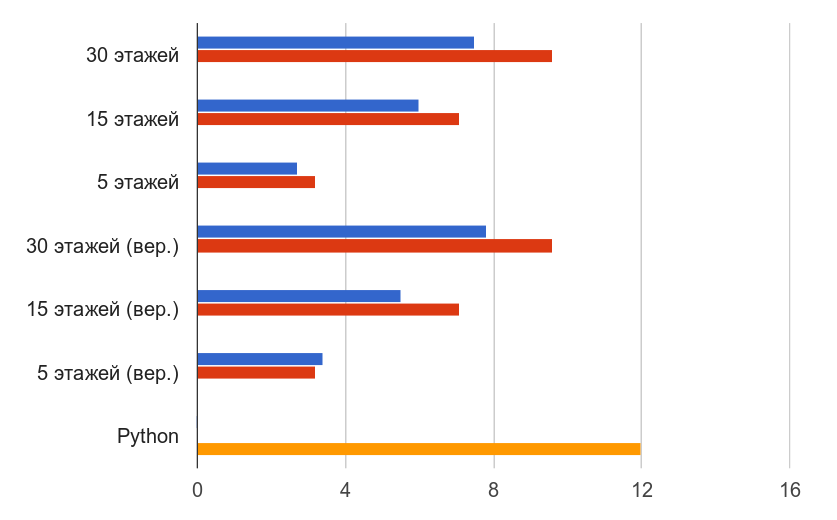
\includegraphics[width=180mm]{src/pictures/projectp1.png}
			\caption{Сравнение по среднему времени ожидания}\label{pt1}
		\end{figure}

		\begin{figure}[h]
			\centering
			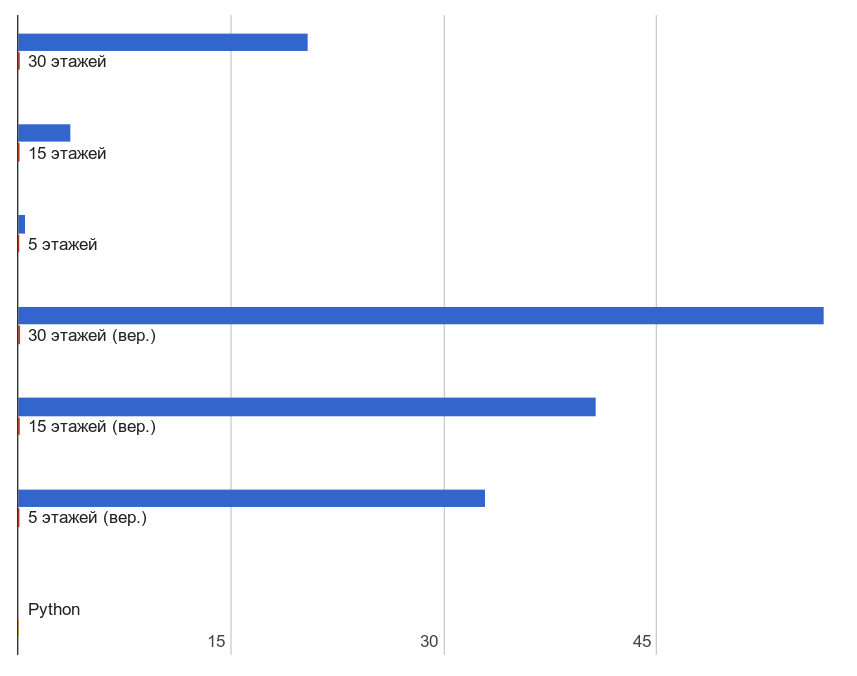
\includegraphics[width=180mm]{src/pictures/projectp2.png}
			\caption{Сравнение по времени выполнения}\label{pt2}
		\end{figure}

	\input{src/spec.tex}
	\chapter{Схема функциональная}
	\section{Схема электрическая функциональная}
	\begin{center}
		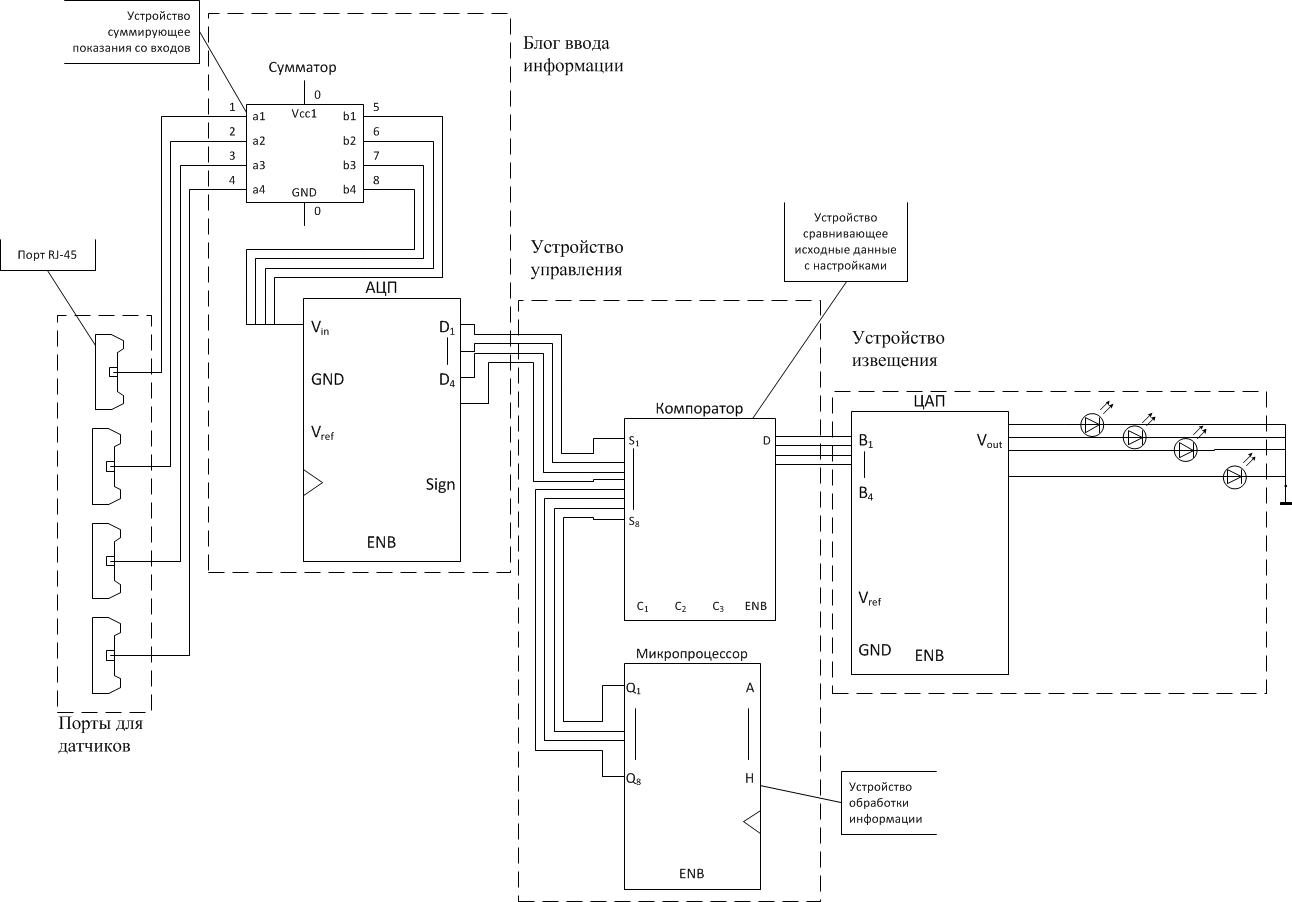
\includegraphics[width=180mm]{src/pictures/schemep1.png}
	\end{center}
\chapter{Схема структурная}
	\section{Схема электрическая структурная}
	\begin{center}
		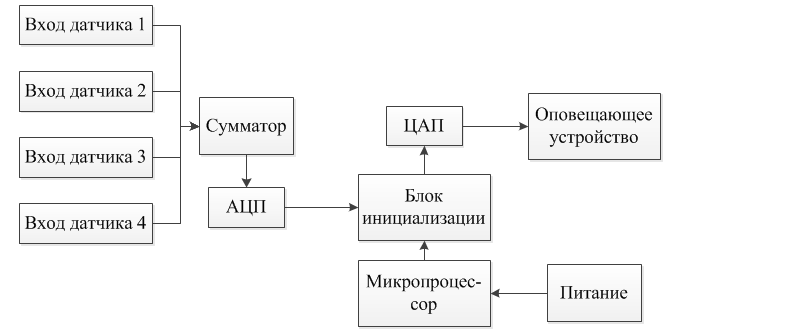
\includegraphics[width=180mm]{src/pictures/schemep2.png}
	\end{center}
\chapter{Схема принципиальная}
	\section{Схема электрическая принципиальная}
		\begin{center}
			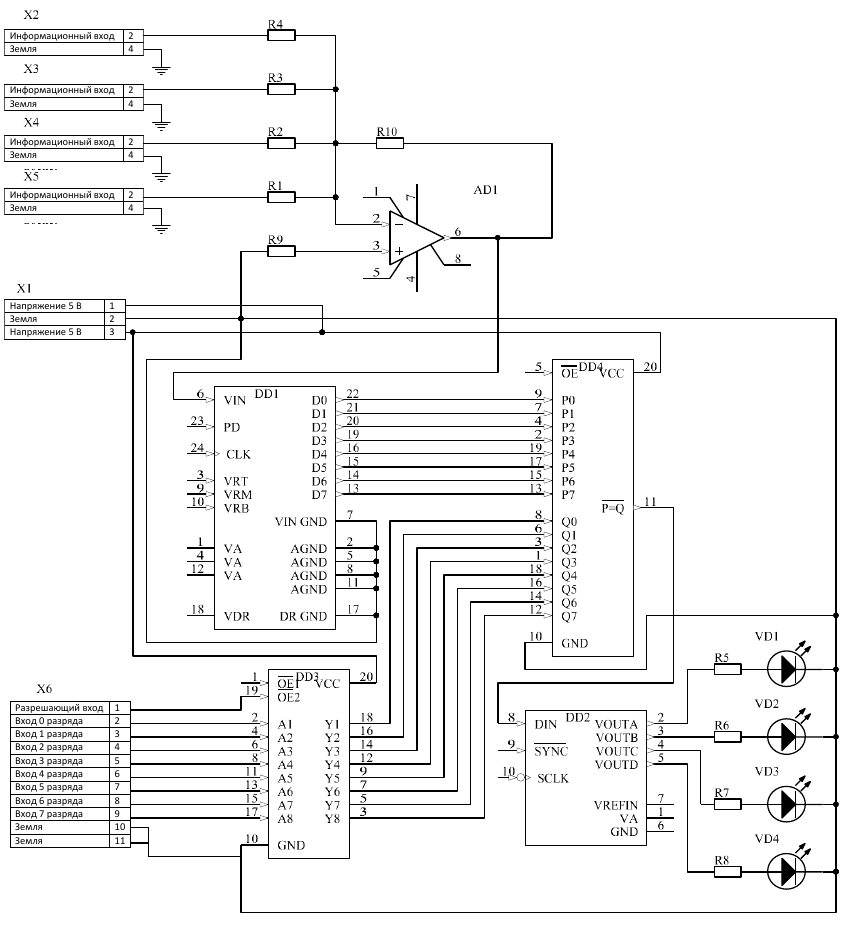
\includegraphics[width=165mm]{src/pictures/schemep3.png}
		\end{center}
		% \newpage
	\section{Перечень элементов}
		\begin{longtable}[t]{@{\extracolsep{\fill}}|l|@{\hskip-14pt}p{0.3\textwidth}|@{\hskip-14pt}p{0.3\textwidth}|l|}
	\caption{Перечень элементов} \label{shcemet1} \\ \hline
	{\No} & Поз. обозначение
		   & Наименование
				& Кол-во   \\ \hline
	1	&	R1-R10	&	Резистор МЛТ, 1 кОм, 0.5 Вт					& 10	\\ \hline
	2	&	X1		&	Разъём для питания розетка С13				& 1		\\ \hline
	3	&	X2-X5	&	Разъёмы для датчика розетка RJ45			& 4		\\ \hline
	4	&	VD1-VD4	&	Диод BL-513-B								& 4		\\ \hline
	5	&	X6		&	Разъём DB9									& 1		\\ \hline
	6	&	DD1		&	Аналого-цифровой преобразователь ADC08L060	& 1		\\ \hline
	7	&	DD2		&	Цифро-аналоговый преобразователь DAC084S085	& 1		\\ \hline
	8	&	AD1		&	Аналоговый сумматор LF411СN					& 1     \\ \hline
	9	&	DD3		&	Регистр 74AC244B							& 1     \\ \hline
	10	&	DD4		&	Компаратор 54AC11520FK						& 1     \\ \hline
\end{longtable}


	\chapter{Чертёж основания}
	\begin{center}
		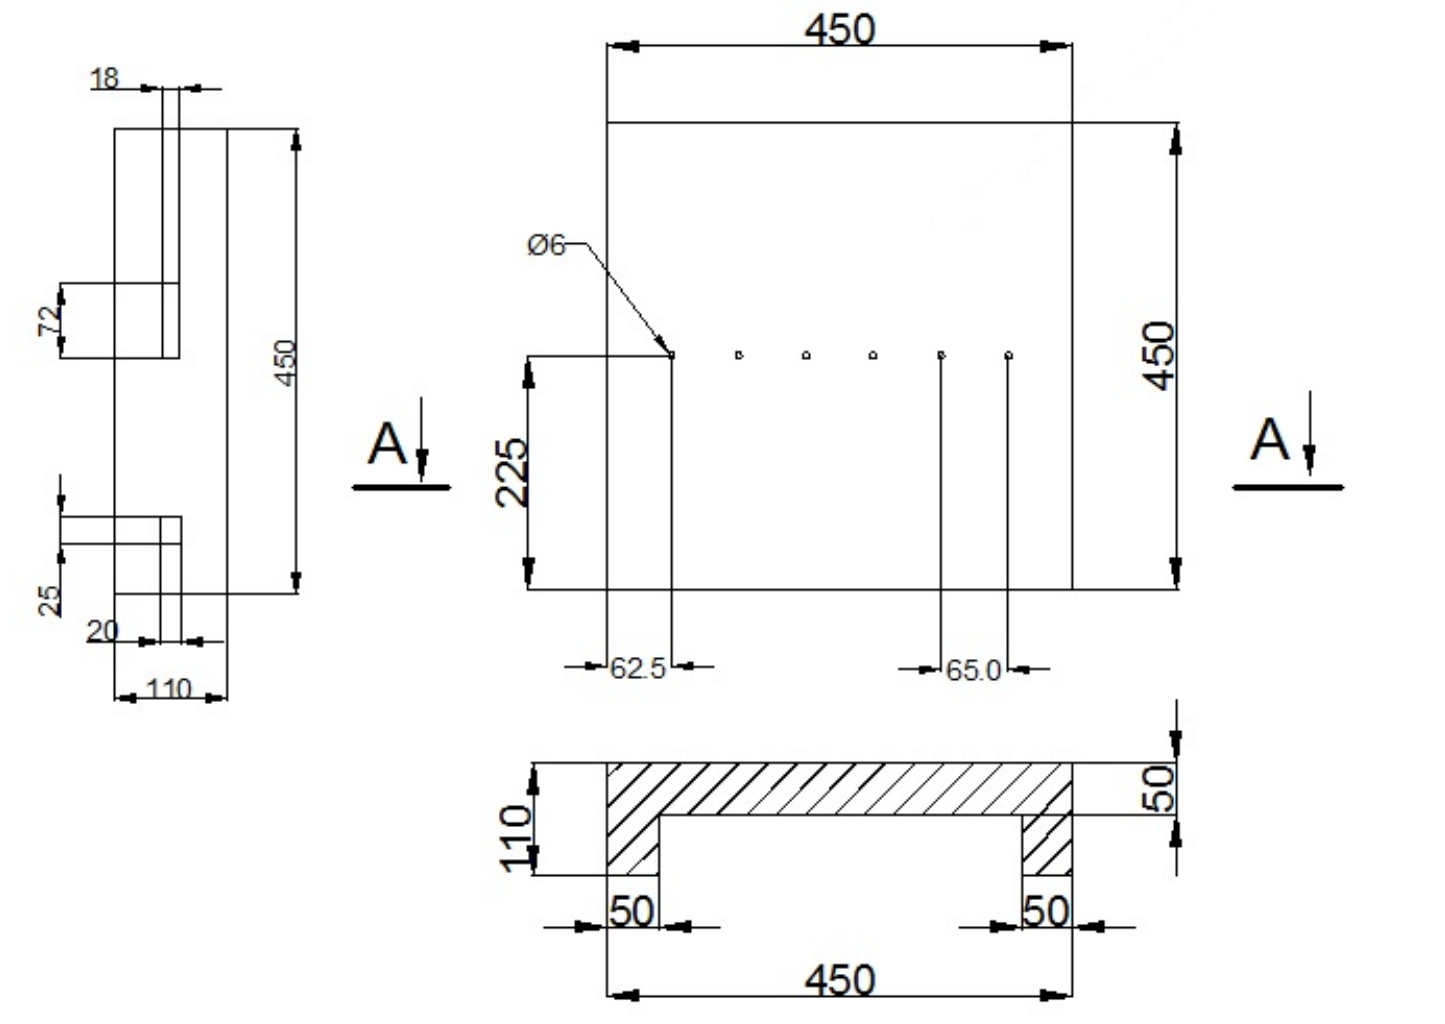
\includegraphics[width=180mm]{src/pictures/drawingp1.png}
	\end{center}
\chapter{Чертёж крышки корпуса}
	\begin{center}
		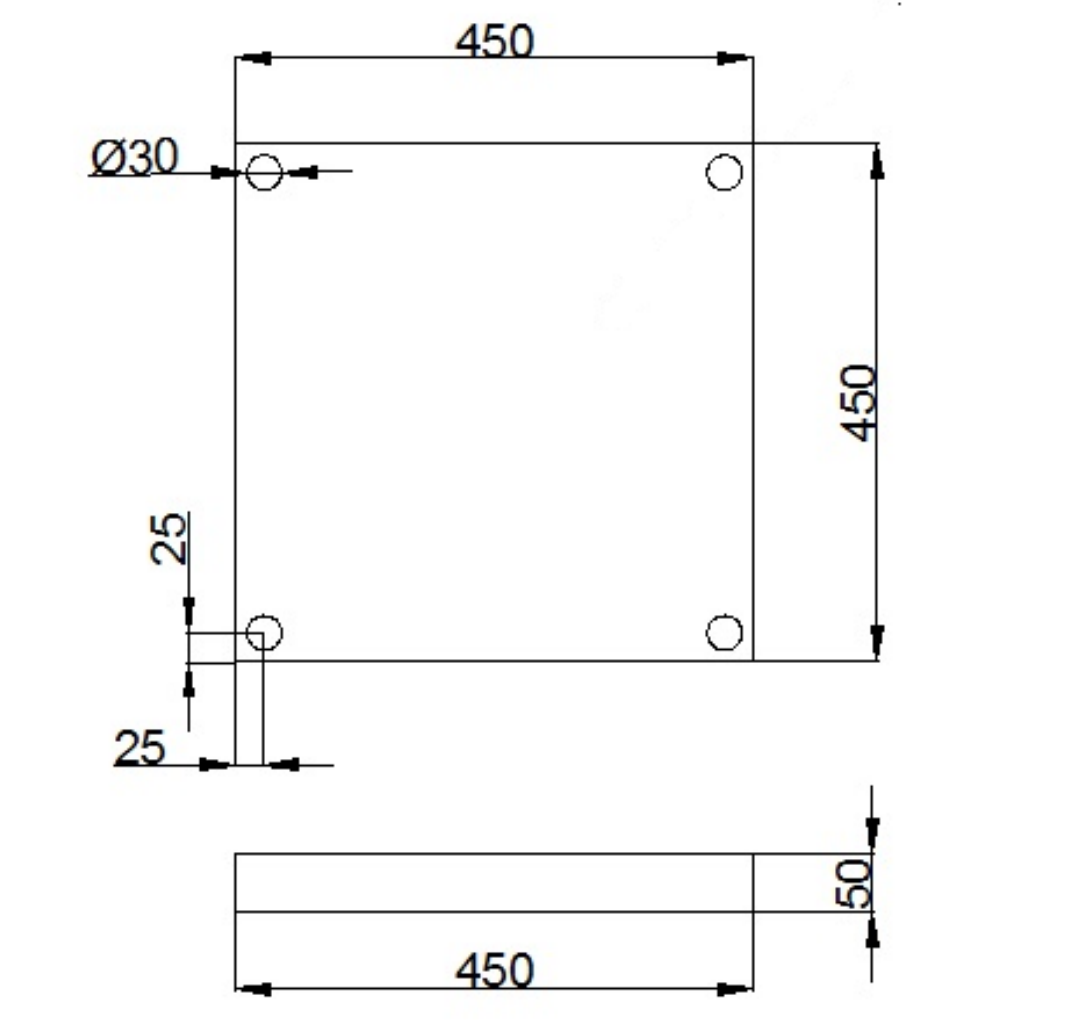
\includegraphics[width=130mm]{src/pictures/drawingp2.png}
	\end{center}
\chapter{Чертёж сборочный}
	\begin{center}
		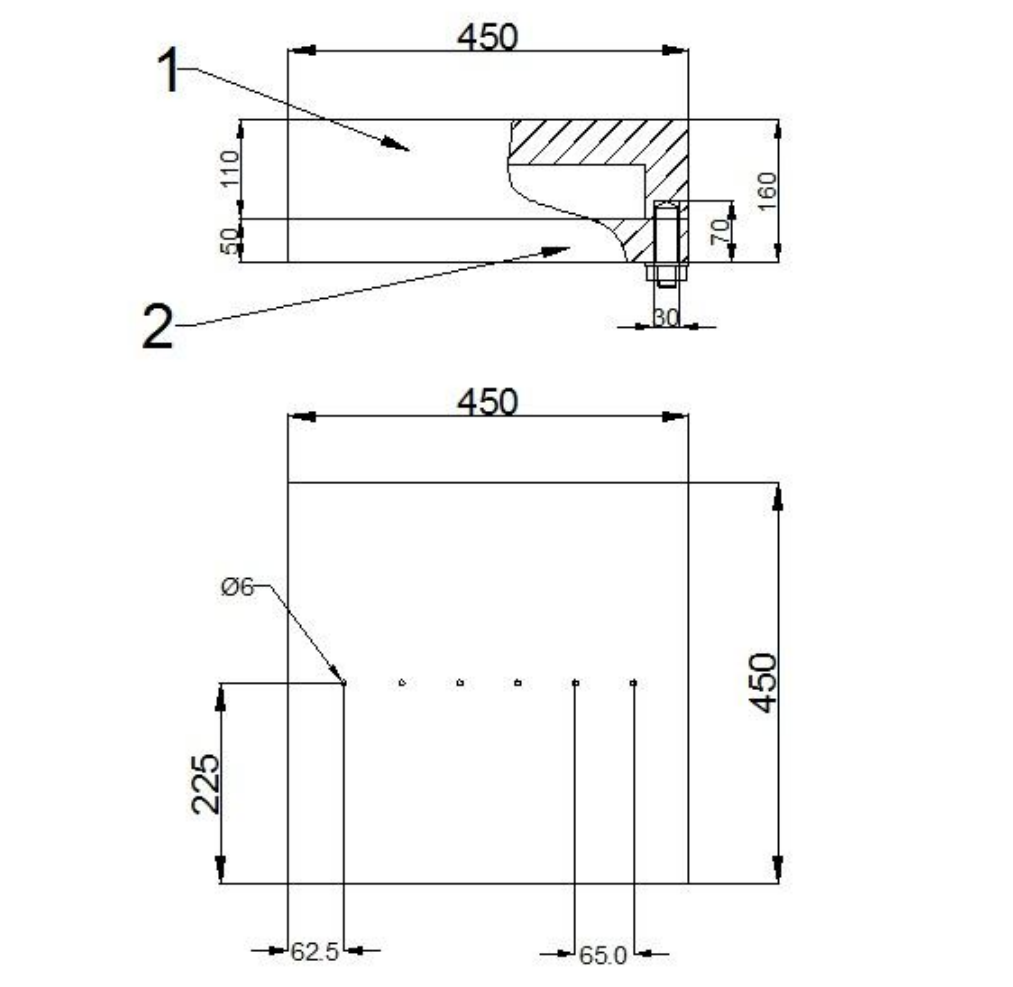
\includegraphics[width=150mm]{src/pictures/drawingp3.png}
	\end{center}

	\chap{Рисунок печатной платы}
	\begin{center}
		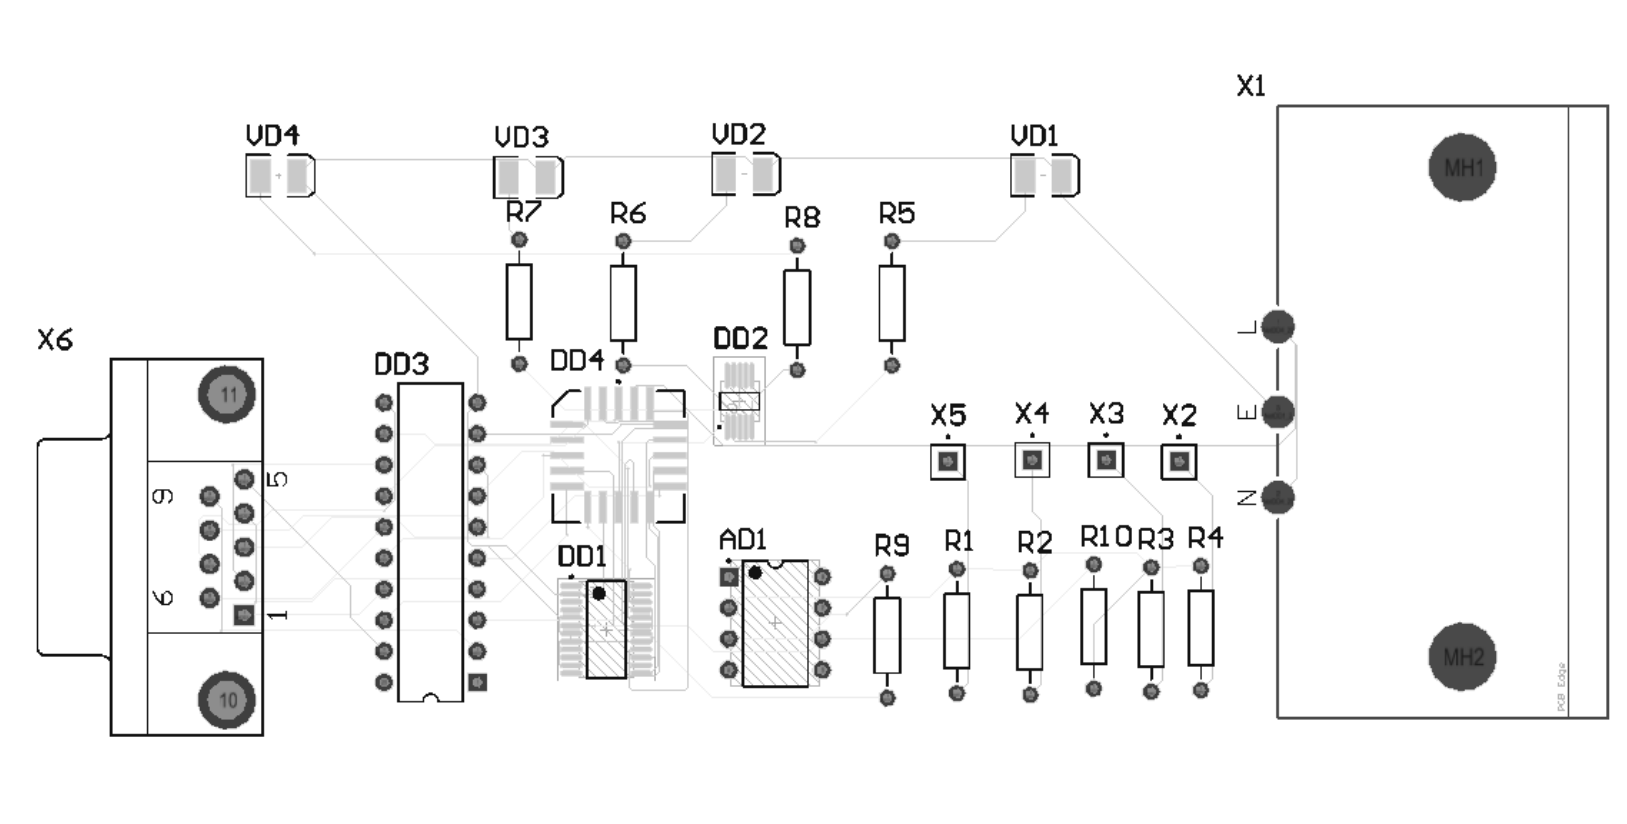
\includegraphics[width=170mm]{src/pictures/picturep1.png}
	\end{center}

	\chapter*{Заключение}\addcontentsline{toc}{chapter}{Заключение}


	\newpage
	% \begin{center}
	% \end{center}
	\bibliographystyle{/home/sava/latex/utf8gost705u}
	\addcontentsline{toc}{chapter}{Список использованных источников}
	\renewcommand\bibname{Список использованных источников}
	\bibliography{biblio}
\end{document}
